\documentclass[a4paper,10pt]{article}

% Hier die Nummer des Blatts und Autoren angeben.
\newcommand{\blatt}{12}
\newcommand{\autor}{Merlin Steuer, Till Schander, Lennart Bergmann}

\usepackage{hci}

\begin{document}
% Seitenkopf mit Informationen
\kopf
\renewcommand{\figurename}{Figure}

\aufgabe{17}

Entwickelt werden soll eine Smartwatch-App, welche es innerhalb einer Smart-Home-Umgebung erlaubt, die Temperatur und Qualität der Luft zu überwachen und zu manipulieren. Überwachte Parameter sind u.a. die Temperatur, die Luftfeuchtigkeit, der Sauerstoffgehalt sowie ggf. Schadstoffgehalt in der Raumluft. Mittels der App sollen mit einfachen Befehlen Belüftungs- und Heizsysteme gesteuert werden können.

\section{Analyse}

\subsection{PACT-Analyse}

\begin{itemize}
    \item Persons: 
        \begin{itemize}
            \item Junge Eigenheimbesitzer
            \item 25-45 Jahre alt
            \item Technikinteressiert und -affin
            \item Besitzer von Smartwatches auf Android- oder iOS-Basis
            \item Besitzer eines vollausgestatteten Smart-Homes
        \end{itemize}
    \item Activities:
        \begin{itemize}
            \item Überwachen der Raumtemperatur
            \item Überwachen der Luftfeuchtigkeit
            \item Überwachen des Sauerstoff- und Schafstoffgehalts der Raumluft
            \item Anzeige eines aggregierten Werts für die Luftqualität
            \item Manipulieren der Umgebungsluft durch Steuerung verschiedener Belüftungs-, Luftbefeuchtungs- und Heizanlagen
            \item Einstellung von Automatismen zum Erhalt einer stabilen Luftqualität
        \end{itemize}
    \item Context:
        \begin{itemize}
            \item Das eigene Heim
            \item Übliche Aufenthaltsorte wie Schlafzimmer und Wohnzimmer. Weniger Augenmerk auf Küche oder Bad
            \item Besondere Nutzung während der Abendstunden zur gemütlichen Zeit
            \item Ggf. für Home-Office-Arbeiter zur Erhaltung einer stabilen Luftqualität bei der Arbeit (Einstellung am PC/Smartphone, Ansteuerung per Smart-Watch)
        \end{itemize}
    \item Technologies:
        \begin{itemize}
            \item Smart-Watch (Android oder iOS) als Steuerungssystem
            \item Diverse Sensoren zum Erfassen der relevanten Luftinformationen
            \item Ein Smart-Home System auf XBee oder ZWave-Basis, welches leicht durch Drittanbieter zu erweitern ist.
        \end{itemize}
\end{itemize}

\subsection{Szenarien}

\subsubsection{Szenario 1}
Peter Klein kommt nach der Arbeit gegen 19 Uhr nach Hause in seine 3-Zimmer Wohnung in der Innenstadt einer großen Metropole. Er empfindet die Luft in seiner Wohnung wegen der exponierten Dachgeschosslage als sehr trocken und heiß.

Um etwas dagegen zu unternehmen schaltet Peter die Klimaanlage seiner Wohnung ein und stellt den Raumluftbefeuchter im Wohnzimmer auf maximale Stufe.

Bevor er ins Bett geht schaltet Peter die Geräte wieder aus um Strom zu sparen und die Lärmbelästigung zu reduzieren.

\subsubsection{Szenario 2}
Annemarie Groß ist Mutter von drei Schulkondern im Grundschulalter. Ihre Kinder haben oft Konzentrationsprobleme, weshalb Sie einen Spezialisten um Hilfe bat, welcher Ihre Luftqualität in der Wohnung bemängelte.

Die Kinder kommen gegen frühen Nachmittag nach Hause. Da Annemarie vormittags daheim ist überprüft Sie mittels diverser Messgeräte die Luftqualität und nimmt entsprechend der Messwerte verschiedene Aktionen in Angriff. Heute ist der Sauerstoffgehalt sehr schlecht und die Schadstoffbelastung hochm, also schaltet Annemarie einen Raumluftionisierer zur Reinigung von Schadstoffen ein und erhöht mittels eines speziellen Apparates den Sauerstoffgehalt der Luft von 16,7 auf 17,1 Prozent.

Seit diese Maßnahmen durchgeführt werden haben Annemaries Kinder deutlich weniger Konzentrationsschwierigkeiten.

\section{Design}

TODO: Skizzen

\section{Implementierung}

TODO: Logo

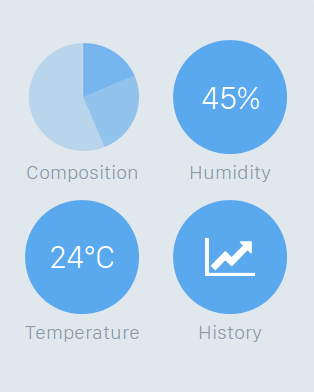
\includegraphics[scale=0.4]{images/home.png}

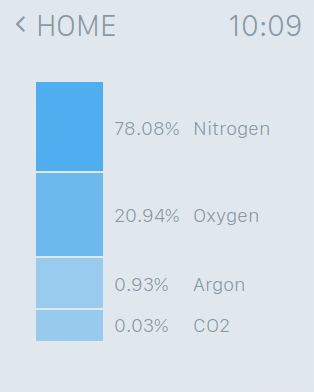
\includegraphics[scale=0.4]{images/composition.png}

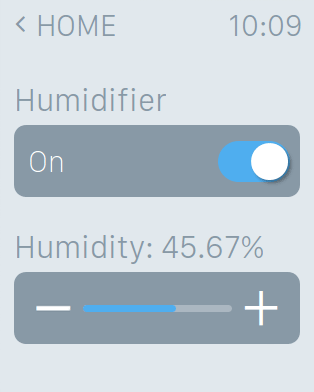
\includegraphics[scale=0.4]{images/humidity.png}

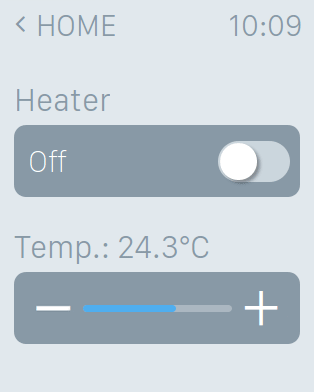
\includegraphics[scale=0.4]{images/temperature.png}

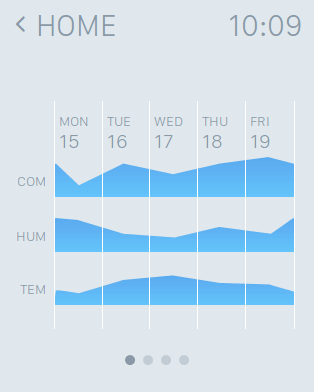
\includegraphics[scale=0.4]{images/history.png}

\section{Evaluation}

\end{document}
